\documentclass[11pt,a4paper]{report}
\usepackage[margin=0.5in]{geometry}
\usepackage[explicit]{titlesec}
\usepackage[dvipsnames]{color}
\usepackage{graphicx}
\usepackage{wrapfig}
\usepackage{lscape}
\usepackage{rotating}
\usepackage{epstopdf}

\definecolor{mygray}{gray}{.75}

\titleformat{name=\section,numberless}[display]
  {\normalfont\scshape\Large}
  {\hspace*{-10pt}#1}
  {-15pt}
  {\hspace*{-110pt}\rule{\dimexpr\textwidth+80pt\relax}{2pt}\Huge}
\titlespacing*{\section}{0pt}{30pt}{10pt}

\titleformat{name=\subsection,numberless}[display]
  {\normalfont\scshape}
  {\hspace*{-10pt}#1}
  {-15pt}
  {\hspace*{-110pt}\rule{\dimexpr\textwidth+30pt\relax}{0.4pt}\Huge}
\titlespacing*{\subsection}{0pt}{20pt}{5pt}


\begin{document}

\noindent\Large\textbf{CM2101 (Human-Computer Interaction)}\\
\noindent\large\textit{Non-assessed Tutorial 3}
\vskip30pt

\section*{Solutions}

\begin{enumerate}
    \item   
        \begin{enumerate}
            \item Column browse\\ 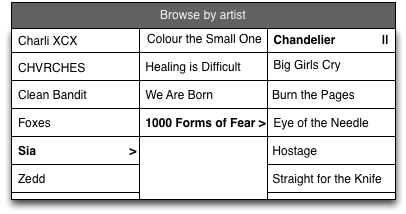
\includegraphics[width=.6\textwidth]{media/column_browse.png}
            \item Filter results\\ 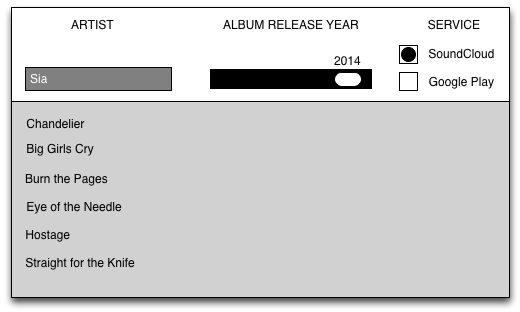
\includegraphics[width=.6\textwidth]{media/filter_results.png}
            \item Master/detail\\ 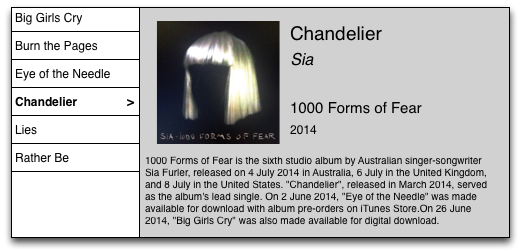
\includegraphics[width=.6\textwidth]{media/master_detail.png}
            \newpage
            \item `Filter results' and `grid of equals'\\ \vskip10pt
                  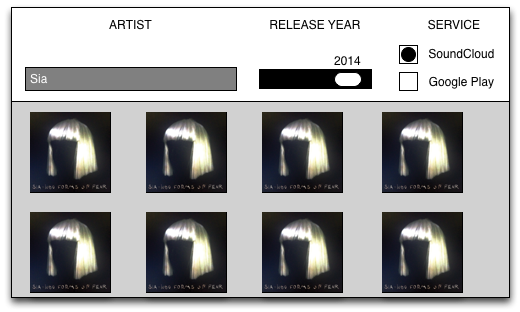
\includegraphics[width=.6\textwidth]{media/filter_results-grid_of_equals.png}\\ \vskip20pt
                  `Column browse' and `master/detail'\\ \vskip10pt
                  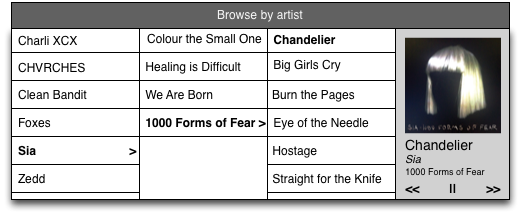
\includegraphics[width=.6\textwidth]{media/column_browse-master_detail.png}
        \end{enumerate}

    \item 
        \begin{itemize}
            \item \textbf{Column browse} - Use of title helps scope displayed data and helps form the plan. Columns navigable by keyboard keys to help in execution. Logical ordering of hierarchy (artist -$>$ album -$>$ song) helps execution and plan (e.g. I know to find the artist first).
            \item \textbf{Filter results} - Labels and inputs make it easy to input information. Easy to plan to find the required song(s), and components are accessible enough to act upon them. Sliding the slider facilitates quick navigation through past albums.
            \item \textbf{Master/detail} - Clear and uncluttered interface makes execution very easy. Songs arranged by alphabetical order makes planning to find a song quick and straight forward. Intentions formed by understanding the interface are clear (either play current song, or find another).
            \item \textbf{Combination} - Both interfaces provide clear routes to complete the task, and thus planning is very easy. Instruction is provided and visual feedback make the next stage of the plan clear. Both interfaces are enhanced by the coupling of patterns - the first allows for easy-visualisation (and thus assisting more with the Gulf of Evaluation), and the second provides the benefits of the clear master/detail view as well as the easy-to-navigate column browse view.
        \end{itemize}

    \item Talk about:
        \begin{itemize}
            \item Improve understandability of interface (cognitive ergonomics)
                \begin{itemize}
                    \item Colours and contrast to help readability (perception)
                    \item Use similarly shaped buttons/action areas for similar tasks to help remember meaning
                    \item Use same icons for similar tasks to help understand meaning
                    \item Arrangement (i.e. address selective attention) to improve evaluation and understanding of information
                    \item Use design patterns to assist in cognitive ergonomics
                \end{itemize}
            \item Use sensible hardware (physical ergonomics)
                \begin{itemize}
                    \item Use good hardware outputs to addist physical ergonomics
                    \item E.g. a bright backlight to help visuals
                    \item E.g. useful sounds to provide alerts
                \end{itemize}
            \item Consider culture (organisational ergonomics)
                \begin{itemize}
                    \item Which colours portray which meaning in your target demographic
                    \item Remember to use neutral colours for important actions if targeting a wide audience
                \end{itemize}   
        \end{itemize}

    \item Could consider these:
        \begin{itemize}
            \item Colour-blindedness
                \begin{itemize}
                    \item Red-green colours hard to distinguish
                    \item Don't use both concurrently
                    \item Don't use one on top of the other
                \end{itemize}
            \item Age-related factors
                \begin{itemize}
                    \item Hardening of lens means blue light harder to perceive
                    \item Avoid solely using blue for text or symbols
                    \item Ensure contrast to support weakening of lens
                \end{itemize}
            \item In general, don't rely solely on colour - use icons and action shapes to convey meaning of action and information.
        \end{itemize}

\end{enumerate}

\end{document}
